\documentclass[a4paper, 12pt]{article}
\usepackage{cmap}
\usepackage{amssymb}
\usepackage{amsmath}
\usepackage{graphicx}
\usepackage{amsthm}
\usepackage{upgreek}
\usepackage{setspace}
\usepackage{color}
\usepackage{pgfplots}
\pgfplotsset{compat=1.9}
\usepackage[T2A]{fontenc}
\usepackage[utf8]{inputenc}
\usepackage[normalem]{ulem}
\usepackage{mathtext} % русские буквы в формулах
\usepackage[left=2cm,right=2cm, top=2cm,bottom=2cm,bindingoffset=0cm]{geometry}
\usepackage[english,russian]{babel}
\usepackage[unicode]{hyperref}
\newenvironment{Proof} % имя окружения
{\par\noindent{$\blacklozenge$}} % команды для \begin
{\hfill$\scriptstyle\boxtimes$}
\newcommand{\Rm}{\mathbb{R}}
\newcommand{\Cm}{\mathbb{C}}
\newcommand{\Z}{\mathbb{Z}}
\newcommand{\I}{\mathbb{I}}
\newcommand{\N}{\mathbb{N}}
\newcommand{\rank}{\operatorname{rank}}
\newcommand{\Ra}{\Rightarrow}
\newcommand{\ra}{\rightarrow}
\newcommand{\FI}{\Phi}
\newcommand{\Sp}{\text{Sp}}
\renewcommand{\leq}{\leqslant}
\renewcommand{\geq}{\geqslant}
\renewcommand{\alpha}{\upalpha}
\renewcommand{\beta}{\upbeta}
\renewcommand{\gamma}{\upgamma}
\renewcommand{\delta}{\updelta}
\renewcommand{\varphi}{\upvarphi}
\renewcommand{\phi}{\upvarphi}
\renewcommand{\tau}{\uptau}
\renewcommand{\lambda}{\uplambda}
\renewcommand{\psi}{\uppsi}
\renewcommand{\mu}{\upmu}
\renewcommand{\omega}{\upomega}
\renewcommand{\d}{\partial}
\renewcommand{\xi}{\upxi}
\renewcommand{\epsilon}{\upvarepsilon}
\newcommand{\intx}{\int\limits_{x_0}^x}
\newcommand\Norm[1]{\left\| #1 \right\|}
\newcommand{\sumk}{\sum\limits_{k=0}^\infty}
\newcommand{\sumi}{\sum\limits_{i=0}^\infty}
\newtheorem*{theorem}{Теорема}
\newtheorem*{cor}{Следствие}
\newtheorem*{lem}{Лемма}
\begin{document}
	\section*{Нелинейные уравнения}
	\subsubsection*{Условия}
	\begin{enumerate}
		\item Отделить один корень уравнения $$2\sin3x = x^2 - 4x + 3.$$ (\hyperlink{t1}{Решение})
		\item Привести к каноническому виду, обеспечивающему сходимость метода итераций, уравнение $$x^7 - 2x - 2=0.$$ Проверить выполнение условий теоремы о сходимости. (\hyperlink{t2}{Решение})
		\item Отделив корень и приведя к виду, удобному для итераций, выбрать начальное приближение, обеспечивающее выполнение условий теоремы о сходимости метода простой итерации уравнения $$2\sin3x = x^2 - 4x + 3.$$ (\hyperlink{t3}{Решение})
		\item Отделив корень, выбрать начальное приближение, обеспечивающее выполнение условий теоремы о сходимости метода Ньютона для уравнения $$2\sin3x = x^2 - 4x + 3.$$ (\hyperlink{t4}{Решение})
		\item Вычислить с точностью $\epsilon=10^{-1}$ наибольший по модулю корень алгебраического уравнения $$2x^3-12x^2+6x +20 = 0.$$ (\hyperlink{t5}{Решение})
		\item Вычислить с точностью $\epsilon=10^{-1}$ корни алгебраического уравнения $$x^3-2x^2+3x +10 = 0.$$ (\hyperlink{t6}{Решение})
	\end{enumerate}
	
	\newpage
	\subsubsection*{Решения}
	\begin{enumerate}
		\item \hypertarget{t1}{}
		 Для решения задачи нам понадобятся утверждения:
		 \begin{enumerate}
		 	\item \textbf{Теорема 1.} Если функция $f(x)\in C[a,b]$ и принимает на его концах значения разных знаков, то на этом отрезке существует по крайней мере один корень уравнения $f(x) = 0$.
		 	Если при этом функция $f(x)$ будет монотонной на отрезке $[a,b]$, то она может иметь только один корень.
		 \end{enumerate}
		 Алгоритм решения следующий: с помощью графического метода отделяется корень, проверяется выполнение теоремы 1.\\\\
		 Для начала построим графики для данного уравнения, так как в данном случае это легко сделать. Определим две функции $$y_1(x) = 2\sin 3x,\quad y_2(x) = x^2 - 4x+3$$ и построим их графики.
		 \begin{center}\begin{tikzpicture}
		 		\begin{axis}[
		 			legend pos = north west,
		 			xlabel = {$x$},
		 			ylabel = {$y$},
		 			minor tick num = 2,
		 			samples=1000,
		 			xmin = -4,
		 			xmax = 4,
		 			ymin = -4,
		 			ymax = 4,
		 			grid = major,
		 			scatter/classes={%
		 				a={mark=o,draw=black}}
		 			]
		 			\legend{$y_1(x)$, $y_2(x)$}
		 			\addplot[blue] {x^2 - 4*x + 3};
		 			\addplot[orange] {2*sin(deg(3*x))};
		 		\end{axis}
		 \end{tikzpicture}\end{center}
		 Приведем исходное уравнение к виду $f(x) = 0$: $$\underbrace{2\sin 3x - (x^2 - 4x+3)}_{f(x)} = 0.$$
		 Область определения функции $f(x)$ совпадает с $\Rm$.
		 Таким образом, уравнение $f(x)=0$ имеет 4 корня на отрезке $[-4,4]$ (и на всей числовой прямой). \\\\
		 Пусть корнем, для которого мы будем искать приближение, будет корень, лежащий слева (однако по аналогии можно найти приближенное значение любого из остальных корней). Этот корень лежит на отрезке $[0; 1]$. Причем из графика видно, что он располагается до точки, в которой функция $y_1(x) = 2\sin3x$ достигает значения $y_1(x) = 2$, то есть до точки $x = \dfrac\pi6$.
		 Таким образом, в качестве отрезка, на котором предположительно располагается исследуемый корень, мы можем взять отрезок $$d = \Big[0; \dfrac\pi6\Big].$$
		 Проверим выполнение условий теоремы 1 корня уравнения на отрезке $d$, для этого вычислим значения функции $f(x)$ на концах отрезка $d = \Big[0; \dfrac\pi6\Big]$:
		 $$f(0) =2\sin0 - 0^2 + 4\cdot 0 -3 = -3 < 0.$$
		 $$f\Big(\dfrac\pi6\Big) = 2\sin \dfrac\pi2 - \dfrac{\pi^2}{36} + 4\dfrac\pi6 - 3 \approx 2 - 0.25 +2-3 = 0.75 > 0.$$
		 Функция на концах отрезка меняет знак, значит хотя бы один корень уравнения $f(x) = 0$ лежит в этом отрезке.\\\\
		 Исследуем функцию на монотонность. Для этого нам нужно оценить значение производной на отрезке. Определим первую производную исследуемой функции: $$f'(x) = 6\cos3x - 2x + 4.$$ Причем эта функция непрерывна на отрезке $d$, то есть $f\in C\Big[0; \dfrac\pi6\Big]$, так как является результатом сложения непрерывных на этом отрезке функций.\\\\
		 Тот факт, что производная не изменяет знак на отрезке докажем аналитически. Разобъем производную на две элементарные функции
		 $$f'(x) = \underbrace{6\cos3x}_{z_1(x)} \underbrace{- 2x + 4}_{z_2(x)}.$$
		 Берем отрезок $d = \Big[0; \dfrac\pi6\Big]$. 
		 \\\\
		 Функция $z_1(x) = 6\cos3x$ является на этом отрезке убывающей функцией по свойствам косинуса. Наибольшее значение $$y_1(0)= 6\cos0 = 6,$$ а наименьшее $$y_2\Big(\dfrac\pi6\Big) = 6\cos\dfrac\pi2 = 0.$$
		 Таким образом, $z_1(x)$ является строго положительной функцией на отрезке $d$. 
		 \\\\
		 Рассмотрим функцию $z_2(x) = -2x + 4$. Она также является убывающей на отрезке $d$ функцией по свойствам линейной функции. Ее наибольшее значение $$z_2(0) = 4,$$ а наименьшее $$z_2\Big(\dfrac\pi6\Big) = -\dfrac\pi3 + 4\approx 3.$$
		 То есть эта функция также является строго положительной на отрезке $d$. 
		 \\\\
		 В итоге функция $f'(x)$ состоит из суммы двух строго положительных на отрезке $d$ функций, а следовательно $$3 \leq f'(x) \leq 10 \Rightarrow f'(x) > 0\quad \forall x \in d=\Big[0; \dfrac\pi6\Big].$$ 
		 Таким образом, мы доказали, что выбранный нами отрезок числовой прямой содержит ровно один корень исследуемого уравнения. На этом решение задачи отделения корней можно закончить и переходить к отысканию приближенных значений корней, лежащих в этих отрезках с помощью указанных методов.
		
		\newpage
		\item 
		\hypertarget{t2}{}
		 Для решения задачи нам понадобятся следующие утверждения:
		 \begin{enumerate}
		 	\item \textbf{Теорема 1.} Если функция $f(x)\in C[a,b]$ и принимает на его концах значения разных знаков, то на этом отрезке существует по крайней мере один корень уравнения $f(x) = 0$.
		 	Если при этом функция $f(x)$ будет монотонной на отрезке $[a,b]$, то она может иметь только один корень.
		 	\item для канонического вида метода простой итерации $x = \varphi(x)$ функция $\varphi(x)$ определена на отрезке \begin{eqnarray}
		 		|x - x_0| \leq \delta,
		 	\end{eqnarray} непрерывна на нем и удовлетворяет условию \begin{eqnarray}
		 		|\varphi'(x)| \leq q < 1,\quad x \in [x_0-\delta, x_0 + \delta],
		 	\end{eqnarray}
		 	где $x_0$ --- начальное приближение.
		 	Тогда метод простой итерации при правильном выборе начального приближения $x_0$ будет сходящимся.
		 \end{enumerate}
		 Алгоритм следующий: отделяем корень, выводим формулу для канонического вида, который будет удовлетворять условию теоремы о сходимости.
		 \\\\
		 Мы имеем $$f(x) = x^7 -2x-2 = 0.$$
		 Попытаемся подбором найти отрезок, на котором находится единственный корень уравнения. Начнем с нуля:
		 $$f(0) = -2 < 0,$$
		 то есть нужно найти точку, в которой $f(x)>0$. Причем уже из формулы $f(x)$ можно заметить, что эта функция будет очень быстро возрастать, то есть мы быстро обнаружим нужную точку. Возьмем единицу:
		 $$f(1) = 1-2-2=-3 < 0,$$
		 то есть единица не подходит. Возьмем двойку:
		 $$f(2) = 2^7 - 4 - 2 > 0,$$
		 эта точка подходит.\\\\
		 Таким образом на отрезке $[1, 2]$ по теореме 1 существует хотя бы один корень уравнения. Докажем единственность, для этого вычислим производную $$f'(x) = 7x^6 - 2,\quad x \in [1,2].$$
		 Из известных свойств функции $x^6=0$, мы можем утверждать, что функция $f'(x)$ на отрезке $[1,2]$ будет возрастающей. Тогда $$f'(1) = 2 \leq f'(x) \leq 7\cdot 2^6 -2 = f'(2),\quad x \in [1,2].$$
		 Теперь необходимо задать формулу канонического вида для итерационного процесса $x = \varphi(x)$. Будем строить ее следующим образом. Возьмем наше уравнение $$f(x) = 0,$$ домножим с двух сторон на постоянную $\lambda$ и прибавим с двух сторон $x$, то есть $$x = \underbrace{x + \lambda f(x)}_{\varphi(x)}.$$ Для сходимости необходимо выполнение условия (2) $$|\varphi'(x)| = |1 + \lambda f'(x)| < 1,\quad x \in [1,2].$$
		 Отсюда $$-2< \lambda f'(x)< 0.$$ Нам известно, что на отрезке $d$ производная имеет положительный знак. Тогда $$-\dfrac{2}{M} < \lambda < 0,\quad M = \max_{[1; 2]}|f'(x)|.$$
		 Причем ранее мы выяснили, что $f'(x) \leq 7\cdot 2^6 - 2 = 446$. Тогда $M = 446.$
		 Тогда мы можем выбрать $$\lambda \in (-\dfrac{1}{223}; 0) \approx (-0.00448, 0).$$ Тогда возьмем, к примеру, $\lambda = -0.00224$ (можно выбрать и другое, но лучше выбирать середину полученного интервала).\\\\
		 Таким образом, мы можем задать функцию для канонического вида: $$\varphi(x) = x -0.00224 \cdot (x^7 - 2x - 2).$$
		 Тогда канонический вид для сходящегося метода итераций задается формулой $$x =  x -0.00224 \cdot (x^7 - 2x - 2).$$
		
		\newpage
		\item 
		\hypertarget{t3}{}
		Для решения задачи нам понадобятся следующие утверждения:
		\begin{enumerate}
			\item \textbf{Теорема 2.}
			(о сходимости метода простой итерации)
			Пусть выполняются следующие условия:\begin{enumerate}
				\item функция $\varphi(x)$ определена на отрезке \begin{eqnarray}
					|x - x_0| \leq \delta,
				\end{eqnarray} непрерывна на нем и удовлетворяет условию Липшица с постоянным коэффициентом меньше единицы, то есть $\forall x, \widetilde{x}$ $$|\varphi(x) - \varphi(\widetilde{x})| \leq q |x - \widetilde{x}| ,\quad 0 \leq q < 1;$$
				\item для начального приближения $x_0$ верно неравенство \begin{eqnarray}
					|x_0 - \varphi(x_0)| \leq m;
				\end{eqnarray}
				\item числа $\delta, q, m$ удовлетворяют условию 
				\begin{eqnarray}
					\dfrac{m}{1-q}\leq \delta.
				\end{eqnarray}
			\end{enumerate}
			Тогда \begin{enumerate}
				\item уравнение $x = \varphi(x)$ в области $(1)$ имеет решение;
				\item последовательность $x_k$ построенная по правилу $x_{k+1} = \varphi(x_k)$ принадлежит отрезку $[x_0 - \delta, x_0 + \delta]$, является сходящейся и ее предел удовлетворяет уравнению $x = \varphi(x)$.
			\end{enumerate}
			\item Выполнение условия Липшица можно заменить более строгим условием 
			\begin{eqnarray}
				|\varphi'(x)| \leq q < 1,\quad x \in [x_0-\delta, x_0 + \delta].
			\end{eqnarray}
		\end{enumerate}
		Алгоритм решения следующий: отделяется корень, выбирается канонический вид и начальное приближение, при котором выполняется теорема 2.\\\\
		\textit{Здесь идет этап отделения корней. В данном файле он пропускается, так как этот этап уже разобран в другом файле}.\\\\
		Из задачи отделения корней уравнения мы имеем, что на отрезке $d = \left[0, \dfrac\pi6\right]$ существует единственный корень уравнения. Приведем исходное уравнение к виду $f(x) = 0$: $$\underbrace{2\sin 3x - (x^2 - 4x+3)}_{f(x)} = 0.$$
		Область определения функции $f(x)$ совпадает с $\Rm$.\\\\
		Нам необходимо задать формулу канонического вида для итерационного процесса $x = \varphi(x)$. Будем строить ее следующим образом. Возьмем наше уравнение $$f(x) = 0,$$ домножим с двух сторон на постоянную $\lambda$ и прибавим с двух сторон $x$, то есть $$x = \underbrace{x + \lambda f(x)}_{\varphi(x)}.$$ Тогда проверим выполнение условия $$|\varphi'(x)| = |1 + \lambda f'(x)| < 1.$$
		Отсюда $$-2< \lambda f'(x)< 0.$$ Нам известно, что на отрезке $d$ производная имеет положительный знак. Тогда $$-\dfrac{2}{M} < \lambda < 0,\quad M = \max_{[0; \frac\pi6]}|f'(x)|.$$
		Оценим значение $M$ аналитически. Вычислим первую производную функции $f(x)$:
		$$f'(x) = 6\cos 3x - 2x + 4.$$
		Разобъем производную на две элементарные функции
		$$f'(x) = \underbrace{6\cos3x}_{z_1(x)} \underbrace{- 2x + 4}_{z_2(x)}.$$
		Берем отрезок $d = \Big[0; \dfrac\pi6\Big]$. 
		\\\\
		Функция $z_1(x) = 6\cos3x$ является на этом отрезке убывающей функцией по свойствам косинуса. Наибольшее значение $$y_1(0)= 6\cos0 = 6,$$ а наименьшее $$y_2\Big(\dfrac\pi6\Big) = 6\cos\dfrac\pi2 = 0.$$
		Таким образом, $z_1(x)$ является строго положительной функцией на отрезке $d$. 
		\\\\
		Рассмотрим функцию $z_2(x) = -2x + 4$. Она также является убывающей на отрезке $d$ функцией по свойствам линейной функции. Ее наибольшее значение $$z_2(0) = 4,$$ а наименьшее $$z_2\Big(\dfrac\pi6\Big) = -\dfrac\pi3 + 4\approx 3.$$
		То есть эта функция также является строго положительной на отрезке $d$. 
		\\\\
		В итоге функция $f'(x)$ состоит из суммы двух строго положительных на отрезке $d$ функций, а следовательно $$3 \leq f'(x) \leq 10 \Rightarrow f'(x) > 0\quad \forall x \in d=\Big[0; \dfrac\pi6\Big].$$
		А тогда $$M = 10.$$
		Тогда мы можем выбрать $$\lambda \in (-0.2; 0).$$ Тогда возьмем, к примеру, $\lambda = -0.05$ (можно выбрать и другое, но лучше выбирать середину полученного интервала).\\\\
		Таким образом, мы можем задать функцию для канонического вида: $$\varphi(x) = x - 0.05 \cdot (2\sin 3x - x^2 + 4x - 3).$$
		Исследуем сходимость построенного итерационного процесса по теореме 2 по соответствующим пунктам:
		\begin{enumerate}
			\item Возьмем $$\Delta = [0; 0.5]\subset d$$ (для удобства вычислений $\Delta$ короче отрезка $d$, но в ином случае лучше брать $\Delta$ не шире $d$).\\\\
			Сперва зададим начальное приближение как середину рассматриваемого отрезка $x_0 = 0.25$. Очевидно на этом отрезке функция определена, непрерывна и дифференцируема (мы показали это ранее). А тогда $\delta = 0.25$.\\\\
			Проверим выполнение условия (4). Для этого продифференцируем функцию $\varphi(x)$:
			$$\varphi'(x) = 1+\lambda f'(x) = 1 - 0.05 \cdot (6\cos 3x - 2x + 4).$$ Ранее мы показали, что $f'(x) > 3$, тогда $$\varphi'(x) < 1 - 0.05 \cdot 3 \leq 0.85 = q.$$
			\item покажем, что выполняется (2):
			Попробуем вычислить значение $m$ аналитически:
			\begin{multline*}
				| 0.25 - (0.25 - 0.05(2\sin0.75 - 0.0625 + 1 -3 ) | = |0.05(2\sin0.75 -1.9375)|\leq\\ \leq |0.05(2\sin\dfrac\pi4 -1.9375)|=|0.05(\sqrt2 - 1.9375)| \approx0.026
			\end{multline*}
			То есть $$m = 0.026.$$
			\item покажем выполнение (3):
			$$\dfrac{0.026}{(1-0.85)}=0.17(3) \leq 0.25$$
		\end{enumerate}
		В итоге мы построили канонический вид для итераций $$x = x - 0.05 \cdot (2\sin 3x - x^2 + 4x - 3)$$
		и выбрали начальное приближение $x_0=0.25$, при котором метод простой итерации будет сходиться.
		
		\newpage
		\item 
		\hypertarget{t4}{}
		Для решения задачи нам понадобятся следующие утверждения:
		\begin{enumerate}
			\item \textbf{Теорема 2.}
			(о сходимости метода Ньютона)
			Выберем начальное приближение так $x^0$, чтобы выполнялись условия сходимости итерационного процесса:
			\begin{enumerate}
				\item Функция $f(x)$ определена и дважды непрерывно дифференцируема на отрезке $$s_0 = [x^0; x^0 + 2h_0],\quad h_0 =- \dfrac{f(x^0)}{f'(x^0)}.$$ При этом на концах отрезка $f(x)f'(x)\ne 0$.
				\item Для начального приближения $x^0$ выполняется неравенство $$2|h_0|M \leq |f'(x_0)|,\quad M = \underset{x\in s_0}{\max}|f''(x)|.$$
			\end{enumerate}
			Тогда справедливы следующие утверждения:
			\begin{enumerate}
				\item Внутри отрезка $s_0$ уравнение $f(x) = 0$ имеет корень $x^*$ и при этом этот корень единственный.
				\item Последовательность приближений $x^k$, $k=1,2,\ldots$ может быть построена по указанной выше формуле с заданным приближением $x^0$.
				\item Последовательность $x^k$ сходится к корню $x^*$, то есть $x^k \xrightarrow[k\to\infty]{}x^*$.
			\end{enumerate} 
		\end{enumerate}
		Алгоритм решения следующий: отделяется корень, выбирается начальное приближение, при котором выполняется теорема 2.\\\\
		\textit{Здесь идет этап отделения корней. В данном файле он пропускается, так как этот этап уже разобран в другом файле}.\\\\
		Из задачи отделения корней уравнения мы имеем, что на отрезке $d = \left[0, \dfrac\pi6\right]$ существует единственный корень уравнения. Приведем исходное уравнение к виду $f(x) = 0$: $$\underbrace{2\sin 3x - (x^2 - 4x+3)}_{f(x)} = 0.$$
		Область определения функции $f(x)$ совпадает с $\Rm$.\\\\
		Вычислим значение производной $$f'(x) = 6\cos 3x - 2x +4.$$	
		Проверим выполнение условий теоремы 2.
		\begin{enumerate}
			\item Выберем отрезок $s_0 = [x_0, x_0 + 2h_0] = \left[0, \dfrac\pi6\right]$. Тогда $$x_0 = 0,\quad h_0 = \dfrac{\pi }{12}.$$
			На этом отрезке функция $f(x)$ непрерывна и дважды непрерывно дифференцируема (это проверяется еще на этапе отделения корней).\\\\
			Проверим, не обращаются ли в ноль значения функции и ее производной на концах отрезка:
			$$f(0) = -3,\quad f'(0) = 10\Rightarrow f(0)f'(0) = -30\ne 0;$$
			$$f\left(\dfrac\pi6\right) = 2-\dfrac{\pi^2}{36} + \dfrac{4\pi}{6} - 3\approx \dfrac34,\quad f'\left(\dfrac\pi6\right) = -\dfrac{2\pi}{6} + 4\approx 3\Rightarrow f\left(\dfrac\pi6\right)f'\left(\dfrac\pi6\right) \approx \dfrac94\ne 0;$$
			То есть первое условие выполнено.
			\item Для проверки условия $2|h_0|M \leq |f'(x_0)|$, $M = \underset{x\in s_0}{\max}|f''(x)|$ необходимо вычислить вторую производную исходной функции:
			$$f''(x) = -18\sin 3x - 2.$$
			Попытаемся оценить максимум модуля второй производной на отрезке аналитически. На отрезке $s_0 = \left[0, \dfrac\pi6\right]$ функия $\sin3x$ является строго возрастающей. Соответственно наибольшее значение она примет на правом конце отрезка $\sin \left(\dfrac\pi2\right) =1$. Тогда наименьшее значение (но по модулю наибольшее) второй производной $$f''\left(\dfrac\pi6\right)=-20.$$
			Тогда $$M = 20.$$
			Проверим, выполнено ли неравенство $2|h_0|M \leq |f'(x_0)|$:
			$$2\cdot \dfrac{\pi}{12} \cdot 20 \not\leq 10.$$
		\end{enumerate}
		То есть \textbf{метод не сходится}, соответственно нужно выбрать другой отрезок $s_0$.\\\\
		Для выбора нового отрезка $s_0$ воспользуемся методом дихотомии, то есть поделим отрезок пополам и выясним, на какой из половинок остался корень, проверив значения на концах отрезка (они должны быть различны):
		$$f(0) = -3 < 0,\quad f\left(\dfrac{\pi}{12}\right) = \sqrt2 - \dfrac{\pi^2}{144} + \dfrac{4\pi}{12} -3\approx -0.6 < 0,\quad f\left(\dfrac{\pi}{6}\right)\approx 0.75 > 0.$$
		Таким образом, корень лежит на отрезке $\left[\dfrac{\pi}{12}, \dfrac{\pi}{6}\right]$ (на монотонность функции мы не проверяем, т.к. от уменьшения отрезка количество корней увеличиться не могло).\\\\
		Снова проверяем условия теоремы о сходимости.
		\begin{enumerate}
			\item Выберем отрезок $s_0 = [x_0, x_0 + 2h_0] = \left[\dfrac{\pi}{12}, \dfrac{\pi}{6}\right]$. Тогда $$x_0 = \dfrac{\pi}{12},\quad h_0 = \dfrac{\pi }{24}.$$
			На этом отрезке функция $f(x)$ непрерывна и дважды непрерывно дифференцируема (это проверяется еще на этапе отделения корней).\\\\
			Проверим, не обращаются ли в ноль значения функции и ее производной на концах отрезка (проверяем только для левого конца)
			$$f\left(\dfrac{\pi}{12}\right) \approx -0.6,\quad f'\left(\dfrac{\pi}{12}\right) = 3\sqrt 2 - \dfrac{\pi}{6} + 4\approx 7.73\Rightarrow f\left(\dfrac{\pi}{12}\right)f'\left(\dfrac{\pi}{12}\right)\ne 0;$$
			То есть первое условие выполнено.
			\item проверим условие $2|h_0|M \leq |f'(x_0)|$, $M = \underset{x\in s_0}{\max}|f''(x)|$.\\\\
			На отрезке $s_0 = \left[\dfrac{\pi}{12}, \dfrac\pi6\right]$ функия $\sin3x$ является строго возрастающей. Соответственно наибольшее значение она примет на правом конце отрезка $\sin \left(\dfrac\pi2\right) =1$. Тогда наименьшее значение (но по модулю наибольшее) второй производной $$f''\left(\dfrac\pi6\right)=-20.$$
			Тогда $$M = 20.$$
			Проверим, выполнено ли неравенство $2|h_0|M \leq |f'(x_0)|$:
			$$2\cdot \dfrac{\pi}{24} \cdot 20 \leq 7.73.$$
			Неравенство выполняется.
		\end{enumerate}
		Таким образом, начальное приближение для сходящегося метода Ньютона равно $x_0 = \dfrac{\pi}{12}$.
		
		\newpage
		\item 
		\hypertarget{t5}{}
		 Для решения задачи методом Лобачевского нам понадобятся следующие формулы:
		 \begin{enumerate}
		 	\item соотношения для коэффициентов: 
		 	\begin{eqnarray}
		 		\begin{cases}
		 			a_0^{(1)} = a_0^2,\\
		 			a_1^{(1)} =2a_0a_2 - a_1^2,\\
		 			a_2^{(1)} = 2a_0a_4 - 2a_1a_3 + a_2^2,\\
		 			\dotfill\\
		 			a_n^{(1)} = (-1)^na_n^2
		 		\end{cases}
		 	\end{eqnarray}
		 	(конкретно эта формула позволяет перейти от итерации 0 к итерации 1, но для перехода от $k$ к $k+1$ соотношения такие же).\\\\
		 	Для нашего случая соотношения будут иметь вид
		 	\begin{eqnarray}
		 		\begin{cases}
		 			a_0^{(1)} = a_0^2,\\
		 			a_1^{(1)} =2a_0a_2 - a_1^2,\\
		 			a_2^{(1)} = - 2a_1a_3 + a_2^2,\\
		 			a_3^{(1)} = -a_3^2
		 		\end{cases}
		 	\end{eqnarray}
		 	\item формула для вычисления корней \begin{eqnarray}
		 		x_i\approx\sqrt[2^k]{ - \dfrac{a_i^{(k)}}{a_{i-1}^{(k)}}},\quad i =\overline{1,n}.
		 	\end{eqnarray}
		 	Конкретно в нашем случае мы можем сразу взять формулу \begin{eqnarray}
		 		x_1\approx\sqrt[2^k]{ - \dfrac{a_1^{(k)}}{a_{0}^{(k)}}},
		 	\end{eqnarray}
		 	т.к. метод Лобачевского возвращает корни в порядке убывания абсолютного значения.
		 \end{enumerate} 
		 \textbf{Замечание.} Метод Лобачевского после прохождения всего цикла возвращает значения корней \textit{по модулю}. Поэтому необходимо подстановкой в исходное уравнение проверить, с каким знаком нужно раскрывать модуль.\\\\
		 Будем обозначать абсолютное значение наибольшего по модулю корня $x$ как $x_1 = |x|$.
		 Для упрощения вычислений преобразуем данный в условии многочлен к приведенному виду (разделим на 2):
		 $$x^3-6x^2+3x +10 = 0.$$
		 Для решения методом Лобачевского удобно составить следующую таблицу (каждый столбец -- это коэффициенты, а в конце значение корня на каждой итерации):
		 $$
		 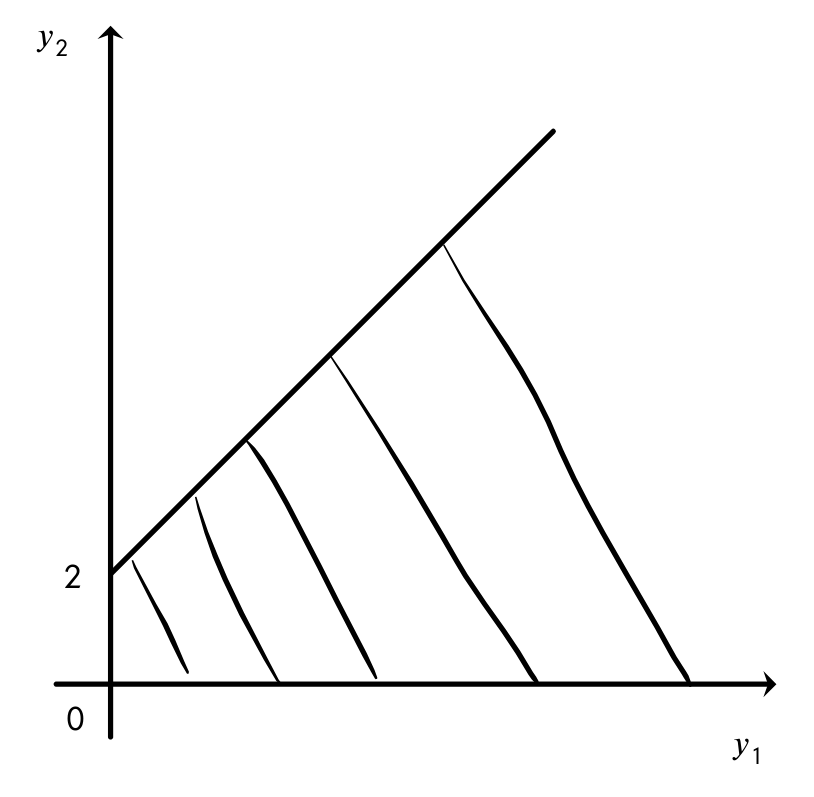
\includegraphics[scale=0.6]{img01}
		 $$
		 Мы переписали коэффициенты исходного многочлена и в последней строке посчитали корень $x_1$ по формуле (3) $$x_1 = - \dfrac{a_1}{a_0}.$$
		 Далее воспользуемся соотношением для коэффициентов (2) и получим новые коэффициенты:
		 $$\begin{cases}
		 	a_0^{(1)} = a_0^2 = 1,\\
		 	a_1^{(1)} =2a_0a_2 - a_1^2 = -30,\\
		 	a_2^{(1)} = - 2a_1a_3 + a_2^2 = 129,\\
		 	a_3^{(1)} = -a_3^2 = -100
		 \end{cases}$$
		 Посчитаем корень по формуле (3) $$x_1^{(1)} = \sqrt{- \dfrac{a_1^{(1)}}{a_0^{(1)}}} \approx 5.4772$$
		 Заносим в таблицу:
		 $$
		 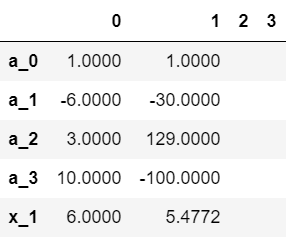
\includegraphics[scale=0.56]{img02}
		 $$
		 Вычислим погрешность: $$|x_1^{(1)} - x_1^{(0)}| = 0.228 > 10^{-1} = \epsilon.$$
		 Так выглядит одна итерация. И пока модуль разности корней не будет меньше $\epsilon$, мы продолжаем итерации.\\\\
		 Далее все действия повторяем. Коэффициенты снова считаем по соотношению (2), а корень теперь вычисляем по формуле (3) как $$x_1^{(2)} = \sqrt{\sqrt{- \dfrac{a_1^{(2)}}{a_0^{(2)}}}}\approx 5.0337$$
		 $$
		 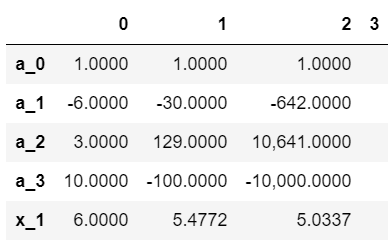
\includegraphics[scale=0.6]{img03}
		 $$
		 $$|x_1^{(2)} - x_1^{(1)}| = 0.4435 > 10^{-1} = \epsilon.$$
		 Сделаем еще одну итерацию. Снова коэффициенты вычисляем по соотношению (2), а корень теперь уже по формуле (3) равен $$x_1^{(3)} = \sqrt[8]{- \dfrac{a_1^{(3)}}{a_0^{(3)}}}\approx 5.0004$$
		 $$
		 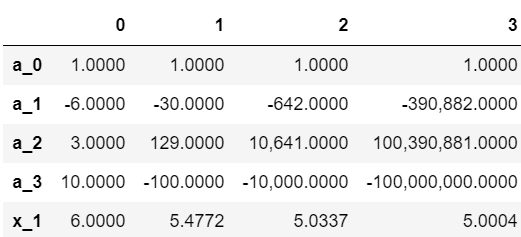
\includegraphics[scale=0.6]{img04}
		 $$
		 $$|x_1^{(3)} - x_1^{(2)}| = 0.0333 < 10^{-1} = \epsilon.$$
		 В итоге мы нашли абсолютное значение наибольшего по модулю: $$|x| = x_1 \approx 5.0$$
		 Необходимо проверить, какое из значений $x=5$ и $x=-5$ является корнем исходного уравнения. Подставим $x=5$:
		 $$125 - 6\cdot 25 + 3\cdot 5 + 10 = 0.$$
		 Можно также проверить и убедиться, что значение $x=-5$ не подходит. Следовательно, $x=5$ --- наибольший по модулю корень исходного уравнения.
		 
		 \newpage
		 \item 
		 \hypertarget{t6}{}
		 Для решения задачи методом Лобачевского нам понадобятся следующие формулы:
		 \begin{enumerate}
		 	\item соотношения для коэффициентов: 
		 	\begin{eqnarray}
		 		\begin{cases}
		 			a_0^{(1)} = a_0^2,\\
		 			a_1^{(1)} =2a_0a_2 - a_1^2,\\
		 			a_2^{(1)} = 2a_0a_4 - 2a_1a_3 + a_2^2,\\
		 			\dotfill\\
		 			a_n^{(1)} = (-1)^na_n^2
		 		\end{cases}
		 	\end{eqnarray}
		 	(конкретно эта формула позволяет перейти от итерации 0 к итерации 1, но для перехода от $k$ к $k+1$ соотношения такие же).\\\\
		 	Для нашего случая соотношения будут иметь вид
		 	\begin{eqnarray}
		 		\begin{cases}
		 			a_0^{(1)} = a_0^2,\\
		 			a_1^{(1)} =2a_0a_2 - a_1^2,\\
		 			a_2^{(1)} = - 2a_1a_3 + a_2^2,\\
		 			a_3^{(1)} = -a_3^2
		 		\end{cases}
		 	\end{eqnarray}
		 	\item формула для вычисления корней \begin{eqnarray}
		 		x_i\approx\sqrt[2^k]{ - \dfrac{a_i^{(k)}}{a_{i-1}^{(k)}}},\quad i =\overline{1,n}.
		 	\end{eqnarray}
		 \end{enumerate} 
		 \textbf{Замечание.} Метод Лобачевского после прохождения всего цикла возвращает значения корней \textit{по модулю}. Поэтому необходимо подстановкой в исходное уравнение проверить, с каким знаком нужно раскрывать модуль.\\\\
		 Для решения методом Лобачевского удобно составить следующую таблицу (каждый столбец -- это коэффициенты, а в конце значения корней на каждой итерации в порядке убывания):
		 $$
		 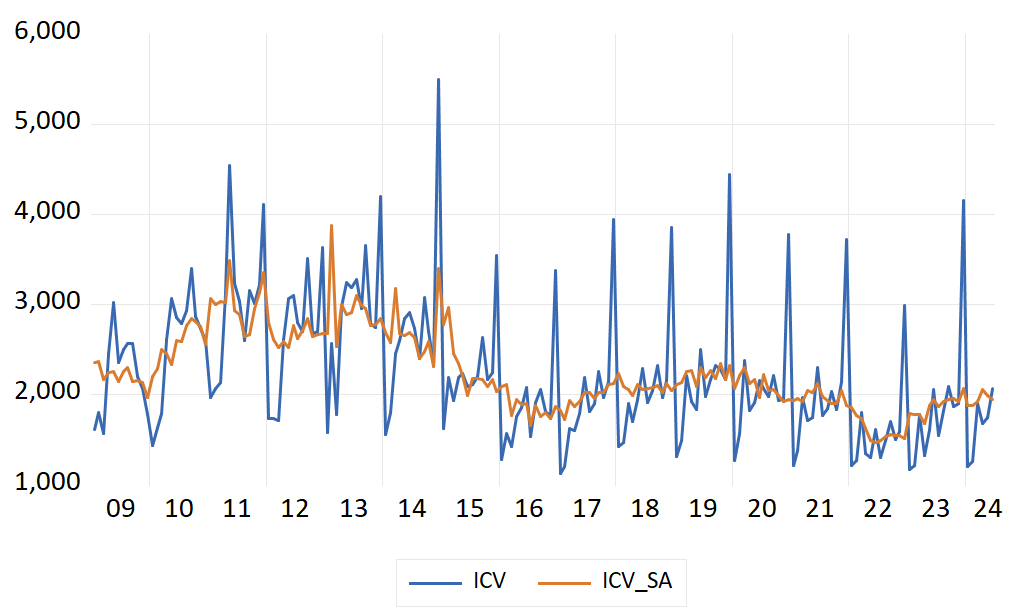
\includegraphics[scale=0.6]{img05}
		 $$
		 где мы посчитали по формулам (3) $$x_1 = - \dfrac{a_1}{a_0},\quad x_2 = - \dfrac{a_2}{a_1}, \quad x_3 = - \dfrac{a_3}{a_2}.$$
		 Считаем коэффициенты и корни из соотношений (2) $$\begin{cases}
		 	a_0^{(1)} = a_0^2 = 1,\\
		 	a_1^{(1)} =2a_0a_2 - a_1^2 = -30,\\
		 	a_2^{(1)} = - 2a_1a_3 + a_2^2 = 129,\\
		 	a_3^{(1)} = -a_3^2 = -100
		 \end{cases}$$
		 По формулам (3)
		 $$x_1^{(1)} = \sqrt{- \dfrac{a_1^{(1)}}{a_0^{(1)}}} \approx 5.4772,\quad x_2^{(1)} = \sqrt{- \dfrac{a_2^{(1)}}{a_1^{(1)}}} \approx 2.0736,\quad x_3^{(1)} = \sqrt{- \dfrac{a_3^{(1)}}{a_2^{(1)}}} \approx 0.8805.$$
		 $$
		 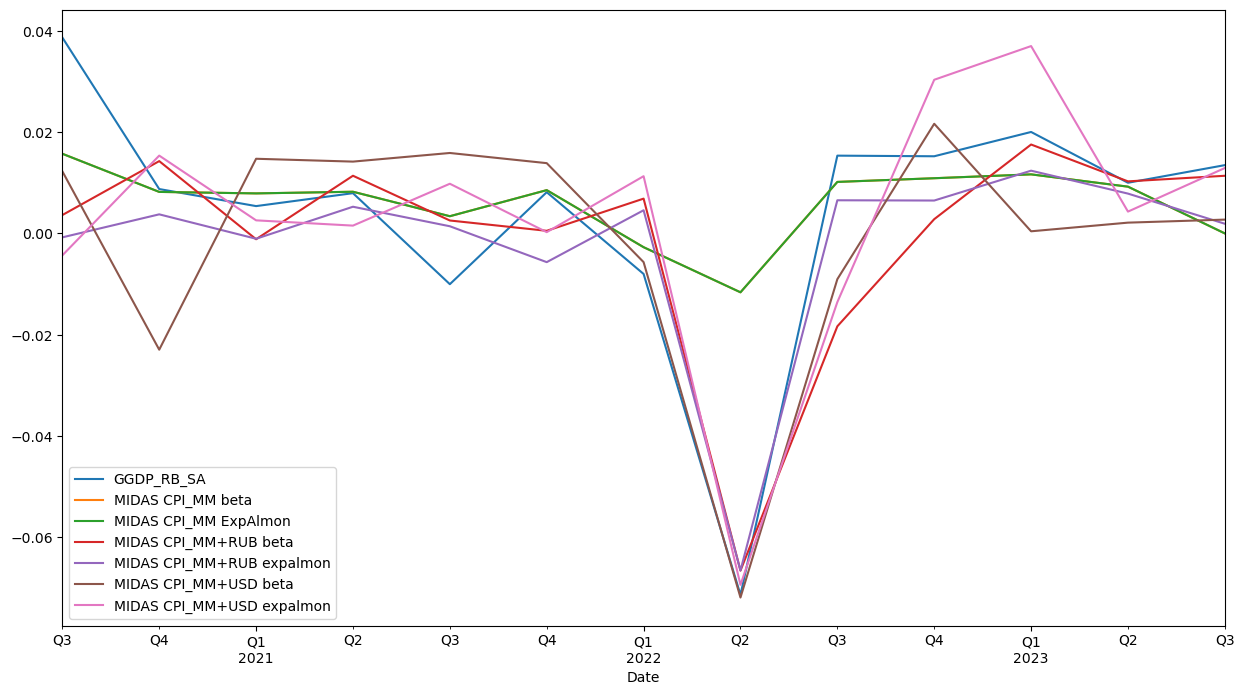
\includegraphics[scale=0.6]{img06}
		 $$
		 Вычислим погрешность. Лучше всего считать разницу для каждого корня, чтобы быть уверенными в том, что каждый корень достиг нужной точности:
		 $$|x_1^{(1)} - x_1^{(0)}| = 0.228 > 10^{-1},\quad|x_2^{(1)} - x_2^{(0)}| = 1.574 > 10^{-1},\quad |x_3^{(1)} - x_3^{(0)}| = 4.214 > 10^{-1}.$$
		 Далее проделываем все то же самое, аналогично случаю отыскания одного корня. Тогда в конечном итоге получается таблица вида:
		 $$
		 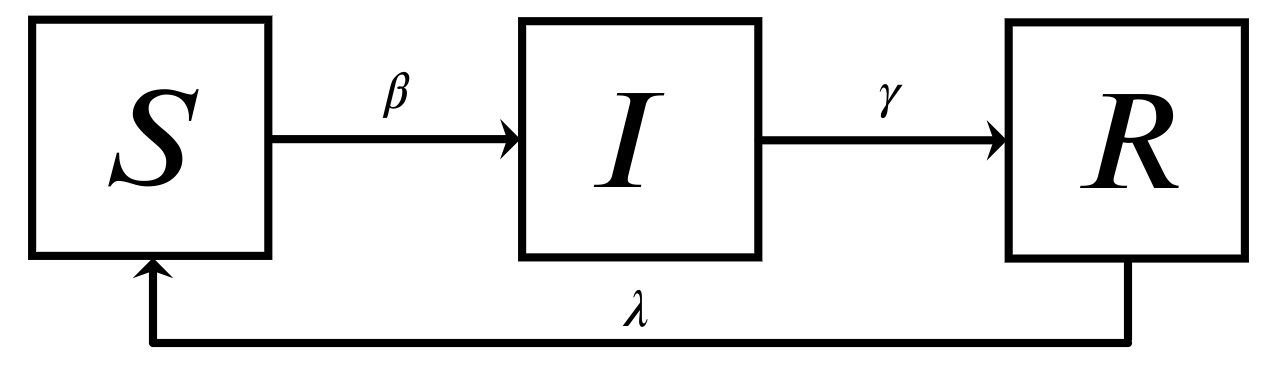
\includegraphics[scale=0.6]{img07}
		 $$
		 Таким образом, округлив, получим значения $$x_1 \approx 5,\quad x_2 \approx 2,\quad x_3 \approx 1.$$
		 Но это абсолютные значения истинных корней. Далее непосредственной подстановкой необходимо выбрать, какие из значений $x=\{-5, -2, -1, 1, 2, 5\}$ действительно являются корнями исходного уравнения.\\\\
		 В данном случае подходят значения $$x=\{1,2,5\}.$$
	\end{enumerate}
	
\end{document} 